\chapter{State of the Art} \label{chap:State of the Art}
This chapter presents the latest research on the topics related to this thesis. In the first section, we introduce reactive systems and different ways to implement them. The second section explains RP and the two libraries from the web domain allowing RP with JavaScript. Traditional debugging tools and techniques along with their limitations with RP are described in the third section. Afterwards, an analysis framework for JavaScript applications called Jalangi is presented in the fourth section. The fifth section presents basic features of Chrome developer tools with a brief guide on writing an extension to add functionality to Chrome DevTools. The chapter finishes with related work from two different aspects.

\section{Implementation of Reactive Systems}
The state is an essential and important part of reactive systems because the state of the system changes as a result of processing events. According to the reactive manifesto \cite{reactiveManifesto}, reactive systems respond in a timely manner even during a failure or variable workload and ensure loose coupling between its components through asynchronous message passing.
Reactive systems are those systems that can react to events (event-driven) and to its users (responsive). We can think of web applications as reactive systems, where events happen to DOM \cite{W3DOM} elements, and result in a change in the state, which can be visible or hidden to the end user \cite{Zanarini:2014:MRS:2637113.2637120}.
Continuously updating the state of systems and the propagation of every single change into systems make the implementation of reactive systems difficult. The manual approach would be to trigger update code after every single change to the state of the system, this is very complex and error-prone. With the manual approach, there will be no separation of concerns and a lot of boiler code would be required to define simple constraints.

\iffalse
\section{Afore Reactive Programming}
In this section, some traditional techniques used to implement reactive systems are presented. The next section describes reactive programming in general and its implementation in web domain in detail.


Before the invention of high-level programming languages such as C or Pascal, programmers had to write computer programs in a machine or assembly language. In the 1980's, object-oriented concepts made high-level programming languages more modularized. An American professor of computer science expressed his idea of the future of programming languages in an article. He stated that, as high-level programming languages free programmers of the complexity of machine language, higher-level programming systems can provide means to understand and manipulate complex systems and components. Considering today's functional and RP paradigms, his dream has come partly true \cite{Winograd:1979:BPL:359131.359133}.
This section will present some programming paradigms used in the past to implement reactive systems. The next sections will have more focus on reactive languages and libraries.
\fi

\subsection{Observer Design Pattern}
The observer design pattern has been used for a long time to implement interactive applications. This pattern does not eliminate the problems of the manual approach to the propagation of changes, but it does modularize the process of propagation of any change to its dependents. The observer pattern defines dependency between objects so that if one object changes its state, all the other dependent objects are notified automatically \cite{Gamma:1995:DPE:186897}. With the observer design pattern, the amount of code for handling events is quite large and scattered, which leads to a complex and error-prone code \cite{Meyerovich:2009:FPL:1639949.1640091}. A report ``Deprecating the Observer Pattern'' \cite{EPFL-REPORT-176887}, proposed a way to minimize the amount of code in an application to handle events by abstracting the logic of event handling as part of a programming language.

\subsection{Aspect-Oriented Programming} \label{subsec:AOP}
Aspect Oriented Programming (AOP) is a technique for expanding the behaviour of objects, methods, and functions without modifying them. AOP allows us to define points in the code at which some update code should be executed. These points are termed as ``pointcuts'' and the update code that executes on matching pointcuts is called ``advice''. Pointcuts are based on events like 'call of a method' or 'begin/end of a method execution' etc.. So when implementing reactive systems, the code responsible for updating the state of the systems can be implemented with AOP. Using AOP, separation of concerns can be achieved with less boiler code as compared to the manual approach. Like many open source JavaScript libraries, dojo\cite{dojo}, jQuery AOP plugin\cite{jqueryaop} and AspectJS\cite{AspectJs} helps one to do AOP with JavaScript. However AOP is not the best choice to implement reactive systems because dependencies still have to be managed manually.

\subsection{Callbacks}
Before the RP paradigm, event handling in interactive applications was done with the help of asynchronous callbacks known as event handlers. 
Instead of blocking program execution while waiting for the result of an asynchronous computation, callbacks are used to receive the results of asynchronous tasks by registering a method that executes as soon as the result of computation is ready. Nesting callbacks to handle multiple asynchronous tasks in a program mostly leads to a well known problem called ``callback hell'' \cite{Kambona:2013:ERP:2489798.2489802} also known as asynchronous spaghetti \cite{SMLI-TR-2007-166}. Callback hell basically is a state of the program that tries to benefit from callbacks but gets too complex to understand, maintain and give reason about that code. Another drawback of using callbacks is that it needs a shared mutable state and event listeners are hard to compose.

\subsection{Promises}
In JavaScript, the term promise is used for a proxy object that represents a future value that is not available initially and yet to be computed in the future \cite{Kambona:2013:ERP:2489798.2489802}.  In other programming languages, a promise may be called future, delay or deferred. Promises are already implemented by some open source libraries with minor differences in syntax include Q, jquery, deferred.js, vow. In JavaScript, promises became standard with the release of ECMAScript version ES6 in 2015 \cite{ecmaScriptPromise}.
Replacing nested callbacks with promises gives more structure to the code, which in turn becomes easier to handle and understand. Because promises are first class objects, they are easily composable \cite{Kambona:2013:ERP:2489798.2489802}.

\subsection{Iterator Vs Observer Pattern}
The iterator pattern enables the consumer to pull data progressively from any data structure, one item at a time. However, in the case of the observer pattern, the producer sends/pushes data to the consumer when data is ready. The consumer gives a callback to the data producer and the producer pushes the data to the consumer using that callback. In the iterator pattern, the consumer decides when to pull data from the producer, while in the observer pattern, its producer decides when the consumer is going to receive data. Both patterns are explained in detail in the book ``Design Patterns: Elements of Reusable Object-Oriented Software by Gang of four'' \cite{Gamma:1995:DPE:186897}. The observer pattern is well-suited for UI events while the iterator pattern is better for traversing different types of collections in a consistent way.

\iffalse
\subsection{Imperative vs Functional programming}
Imperative programming paradigm prescribes the computer what to do, and step-by-step procedures are used. It is closer to machine language. In imperative programming, we commonly use the if-structure, loops, functions etc. C and Java are the examples such programming languages. Imperative programming is easy to understand and debug. Normally it has objects and defined state variables, but the code can be lengthy and hard to scale.
In imperative programming, there is freedom of changing values anytime, but the consequences of those changes must be dealt manually \cite{Edwards:2009:CR:1639950.1640058}.

In functional programming paradigm, we describe the end results, and use function calls, higher order functions, recursion etc.. Pure functional approach has no memory/IO side effects. It requires less code, which is easy to scale. The functional programming paradigm is not well suited for simple tasks. The code in functional approach is a bit complex to understand. In functional programming, the task is achieved by calling a function without knowing the details of how operations are performed. Scala, Haskel and Lisp are based on the functional programming paradigm.
\fi

\section{Reactive Programming}

In recent years, advancements in technology and high expectations from application users has changed software applications dramatically and resulted in more interactive applications.
Handling large amounts of data, quick response times, not having any downtime and being able to run the application on various platforms are some of the current applications requirements \cite{reactiveManifesto}. Applications need to be more responsive to the events happening outside and within an application environment like never before. Users tend to regularly use responsive systems while non-responsive systems rapidly lose their users. To fulfil the above mentioned requirements, sequential and imperative programming techniques are not enough because of unpredictable behaviour of events and their effects. Before the RP model, any changes in state, its effects and order of performed actions were managed by programmers manually. This was very complex and likely to fail or cause errors in results \cite{Edwards:2009:CR:1639950.1640058}.
Reactive programming came into existence as a programming model that assists in developing event-driven and interactive applications. RP provides abstractions for representing values that change over time, event handling and state management. Time-changing values, data flow management, propagation of change and tracking of dependencies are key concerns of this paradigm \cite{Margara:2014:WDD:2611286.2611290}. The programmer specifies constraints among the variables and then all the required operations to fulfill those constraints are performed by RP runtime \cite{6840828}. The RP model is similar to the spreadsheet model in the sense of handling computation dependencies automatically, like changing the value of one cell can effect other cells automatically in a spreadsheet \cite{Bainomugisha:2013:SRP:2501654.2501666}. In RP if some variable is defined as a time changing value, then it means every time there will be a change in the value of that variable, reactive language or library will automatically propagate that change to all parts of the program that depends on this particular variable.
For example, if we have expression ``var a = b + c;'' traditional programming languages will treat this expression as just an assignment of the sum of values of b and c, while in RP this is treated as a constraint. So, whenever the value of b or c get changed, the value of a will be updated automatically.
By using RP, the composition and comprehension of the software improves as compared to the traditional observer
pattern \cite{Meyerovich:2009:FPL:1639949.1640091,Bainomugisha:2013:SRP:2501654.2501666,EPFL-REPORT-176887}. Design benefits of RP could be verified with preliminary empirical results of REScala and more recently, the claimed advantage of RP about better comprehension also has been empirically evaluated in detail \cite{7827078}.
This programming model has more emphasis on scalability and responsiveness, so we can say that RP is a programming model that help us to build a scalable architecture that is resilient and quick to react to any change. An event-driven programming model has more focus on handling single events while RP focuses on data flows and propagating changes all over.
Thus far, most reactive languages have been implemented on top of functional programming paradigm, hence, this is also known as functional RP.

Event-based languages and abstraction in order to represent reactive values on top of existing languages are two different approaches used to implement reactive applications \cite{Salvaneschi:2014:RBO:2577080.2577083}. 
Ptolemy \cite{Rajan2008}, EventJava \cite{Eugster2009}, EScala \cite{Gasiunas:2011:EME:1960275.1960303} and DominoJ \cite{Zhuang:2013:MSS:2451436.2451460} are all examples of event-based languages that support the event on the language level. Events are composable and update code can be easily separated from the main code to achieve a basic design principle of separation of concerns. Manual registration of event handlers and dependency management makes this approach an unfavourable choice for reactive applications.
Reactive languages have direct representation of reactive values and allow composition by dedicated abstraction. Constraints are defined and runtime of language take care of propagating any change to all dependents.
Fran \cite{Elliott:1997:FRA:258949.258973} implements the concept of reactive values as Haskel library. It is a collection of data types and functions for composing richly interactive and multimedia animations. Other reactive languages like Scala.React \cite{EPFL-REPORT-176887}, FrTime \cite{Cooper2006} also implement the same concepts in a new fashion.
The next section focuses on this second approach and more specifically, the reactive libraries in the web domain which are a central topic for this thesis

\subsection{Reactive Programming with JavaScript}
JavaScript is a well-known programming language for developing client-side web applications and was ranked as the seventh overall most popular
programming language in February 2017 \cite{TiobeIndex}. JavaScript is considered to be a dynamic programming language because it provides features at runtime that non-dynamic programming languages provide during compile time. 
Treating functions as objects, allowing insertion and evaluation of code at runtime using 'eval', providing an interface to make requests to web servers and manipulating DOM at runtime make JavaScript a dynamic programming language \cite{White2010}. Ajax revolution in 2005 further increased the popularity of JavaScript as a significant programming language. Competition between browser vendors (Mozilla, Microsoft, Apple, Opera, and Google) as resulted in vast improvements in JavaScript performance \cite{cantelon2014node.js}. Ryan Dahl, the author of Node.js \cite{NodeJs}, was looking to build non-blocking I/O server platform. He tried C and Lua as the programming language for his project but eventually turned to JavaScript because it lacked a robust input/output model (meaning that he could write his own new one) and had the fast and fully programmable V8 runtime readily available \cite{9780321910578}. Closures and first class functions in JavaScript also make it a powerful match for his project \cite{teixeira2012professional}. In 2009, Ryan Dahl presented an early version of Node.js library at JSConf in Berlin \cite{JSConfNodeJS}. It is built on Google Chrome's V8 JavaScript runtime engine and allows programmers to do server side programming using JavaScript. JavaScript applications are portable as most of the modern day devices have a browser that runs JavaScript applications \cite{Richards:2010:ADB:1809028.1806598}.
Web applications nowadays are not static HTML pages anymore. They have become more interactive and complex, containing asynchronous behaviours \cite{6068340}. Before RP, the above mentioned requirements were managed with the help of callbacks, but those are difficult to handle and error prone. To manage the complexity of modern day interactive web applications, some JavaScript libraries have been developed in recent years to implement RP paradigms. We will discuss the two most commonly used JavaScript reactive libraries in detail as these will be the main focus of this thesis.

\subsection{ReactiveX and RxJS}
ReactiveX is basically a pool of libraries based on different well-known programming languages like Java, PHP, JS etc.. It provides libraries on top of these different programming platforms to add abstraction to those languages and enable programming in a more declarative and reactive manner. Sometimes the term functional RP has been misused for ReactiveX library, but functional reactive programming is a bit different. The major difference between these two is that functional reactive programming operates on values that change continuously over time while ReactiveX operates on discrete values that are emitted over time \cite{reactivex}. 
The Reactive extension for JavaScript(RxJS) is a set of libraries to develop asynchronous and event-based programs. Basically, RxJS is composed of three components, namely Observables, Operators, Schedulers. Observables are used to represent asynchronous data streams. A stream can be defined as a sequence of ongoing events ordered in time. Mouse movement, clicks, HTTP requests and UI events are examples of a stream. Operators are used to transform those event streams from one form to another and use schedulers to
handle concurrency in between event streams \cite{rxjs}.

\subsection{Important Concepts of RxJS}
\subsubsection{RxJS Reactive Pattern}
In ReactiveX anything can be represented as a stream of data or events which are called Observable. Later those streams can be functionally transformed to another stream or can be combined with other streams to make a new stream. Finally, each stream can be consumed by any number of subscribers. An observer subscribes to an observable and reacts to items emitted by an observable. This concept ensures concurrency because the observer does not need to block itself while waiting for data from an observable. The marble diagram is a great way to visualize this pattern. In figure~\ref{fig:rxjs-reactive-pattern}, a marble diagram is used to explain observables and transformation of observables to another form.
\begin{figure}[!h]
	\centering
	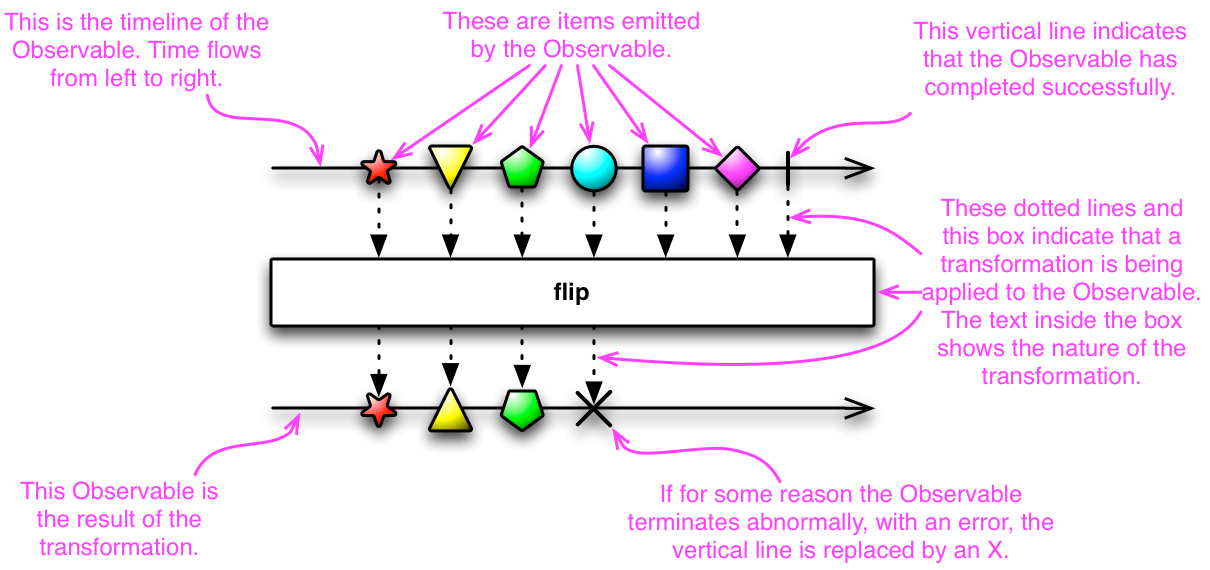
\includegraphics[scale=0.5,trim=0 0 0 0]{gfx/rxjs-reactive-pattern2.png}
	\caption{Reactive pattern \protect\cite{ReactiveXobservable}}
	\label{fig:rxjs-reactive-pattern}
\end{figure}

\subsubsection{Observable and Observer}
As we have already mentioned, the Observable pattern is the 'push' equivalent of the Iterator pattern. However, the Gang of Four's Observer pattern \cite{Gamma:1995:DPE:186897} still misses two key semantics of the Iterator pattern. The first one is the producer not signalling to its consumer that there is no more data available. The second is that the producer is not informing the consumer if an error takes place. With observable type, an observable calls its observer's onCompleted method to implement first semantic and calls its observer's onError method for the second missing semantic. With these additions, the iterable and observable types becomes more equivalent to each other. The only difference between them is the direction in which data flows. This equivalence makes it possible to perform any operation on observable that we can perform on iterable \cite{reactivex}.
The observable is the basic building block of RxJS. It is the name of another abstract data type just like an array and other collections in programming languages. It represents any set of values over any amount of time. An Observable contains a sequence of values that a data producer pushes to the consumer. An Observable can also signal to its listener that it has been completed and will not send any more data. Using an array, all the data is stored in memory and using the Observable, there is no data stored in memory and items arrive asynchronously over time. We can also name the observable object as a provider because it represents the object that sends notifications to the observer object.
An Observable gives us an object that represents an event stream and we can use that object to perform different methods on that object, as can be done with an array. For example, we can traverse an observable like we can traverse an array. In RxJs, the Observable can hot or cold. Hot observable starts emitting values as soon as it has been created and cold observable starts emitting data when an observer subscribe to it.

\subsubsection{Operators}
\label{subsec:Operators}
Besides extending the observer pattern to support sequences of data and/or events, ReactiveX provides a large number of operators that allow you to compose sequences together declaratively while abstracting away concerns about things like threading, synchronization and concurrency. RxJS provides a bundle of operators that we can apply on observables. An operator takes one observable as input and generates another observable as output. When an operator is called, it does not change the existing Observable instance. Instead, it returns a new Observable, which has different properties then the source observable. A list of operators with their details is available in the reactiveX online documentation \cite{reactivexOperators}. Most of these operators operate on observable and produce another observable which make it possible to chain operators one after another.

\subsubsection{RxJS Code Structure}
In general, we can divide RxJS code into three parts. The first part defines and creates a source observable. The second part involves applying different operators to transform the source observable into the desired observable. Lastly, the desired observable has to subscribe in order to receive emitted values from the desired observable. Let's examine the code structure of RxJS with a simple example in Listing ~\ref{lst:RxJS_Simple_Example}. As we have already seen that the observable is a collection of values over time, we need to define and create an observable before using it. RxJS library gives the possibility to convert single or multiple values, arrays, events, and callbacks into observables. We can also create our own observable by wrapping any functionality that produces values over time.
\begin{lstlisting}[language=JavaScript, caption=RxJS Simple Example, label={lst:RxJS_Simple_Example}]
// 1. Srouce Observable Creation
var sourceObservable = Rx.Observable.interval(1000);
// 2. Transformation by applying different operators
var transformedObservable = sourceObservable.map(function(x) {
		return x * 10;
	})
	.filter(function(x) {
		return x !== 20
	})
	.take(5);
// 3. Subscribe to desired Observable 
var subscription = transformedObservable.subscribe(
	function(x) {
		console.log('Next: ' + x);
	},
	function(err) {
		console.log('Error: ' + err);
	},
	function() {
		console.log('Completed');
	});
// OUTPUT
Next: 0
Next: 10
Next: 30
Next: 40
Next: 50
Completed
\end{lstlisting}
In the example code at line 2 'sourceObservable' is defined as observable using 'interval' operator. Interval operator creates an observable sequence that produces a value after each period. In this case, it emits a sequence of integers spaced by 1000 milliseconds. In line 4 to 10, three operators are chained together to get the desired observable as 'transformedObservable'. Map operator is applied to sourceObservable, that multiplies every emitted value from source observable with 10. So our source observable is supposed to emit values like 0,1,2,3,4.... and after applying map operator our observable will become 0,10,20,30,40..... . There is a filter operator next to map operator in the chain that filters value of 20 from its source observable. After applying the filter operator emitted values are supposed to be 0,10,30,40... The last operator in the list is the take operator that restricts the emitted values to a defined number, in this case to 5.
After transforming the source observable to our desired observable we need to subscribe to our transformed observable. Line 12 to 21 in the example code contains the subscription. Subscribe method take three callbacks, the first one executes whenever a new value emitted by the observable, the second callback is for error handling and executes in the case of any error occuring and the third callback is executed to signal that the observable has been completed and will not emit values anymore. Line 22 to 28 displays the output of the example code.


\subsection{Bacon.js}
Bacon.js is a functional reactive programming library for JavaScript that assists in dealing with the asynchronous nature of JavaScript code. It is comparable to Underscore.js \cite{Underscorejs}, which is a JavaScript library which provides a collection of useful functional programming utilities for common tasks like map, filter, invoke etc..
Underscore.js is for data which is available already like arrays. Bacon.js turns the way  in which individual events are handled with imperative programming model into a functional programming model and works on events streams. So using this library will reduce the complexity of handling events individually into code that will look more logical, easy to understand and functional.

\subsubsection{EventStream and Property}
In Bacon, these are two flavors of Observables. EventStreams and Property are two basic concepts of Bacon.js that are basically known as events and behaviours in the literature of FRP.
EventStreams are sources of events. For example mouse clicks, keyboard events can be modeled into an EventStream object. EventStreams are composable. So we can combine several EventStream objects to create another EventStream.
Property which is also known as behaviours and signals, is an abstraction for the values that vary over time \cite{GithubFRP}.
Properties are very similar to EventStreams and share most of the functionality with EventStream but Property also has the concept of current value and we can create a Property from an event stream by using toProperty or scan method \cite{BaconProperty}.

\subsubsection{Bacon Example}
\begin{lstlisting}[language=JavaScript, caption=Bacon.js Example , label={lst:Bacon_Simple_Example}]
var arr = [1, 2, 3, 4, 5, 6, 7, 8, 9, 10];
var baconSourceStream = Bacon.sequentially(1000, arr);
var baconFilteredEvenStream = baconSourceStream.filter(function(x) {
	return x % 2 == 0;
});

baconFilteredEvenStream.onValue(function(val) {
	console.log('Next: ' + val);
});

baconFilteredEvenStream.onEnd(function() {
	console.log('Completed');
});
baconFilteredEvenStream.onError(function(err) {
	console.log('Error: ' + err);
});

// OUTPUT
Next: 2
Next: 4
Next: 6
Next: 8
Next: 10
Completed

\end{lstlisting}

The example code is a simple code written using the bacon.js library and is very similar to the RxJS example presented earlier.
Line 2 uses the method 'Bacon.sequentially' to create a source event stream containing values from a given array delivered one by one with a given interval in milliseconds. So after every 1000ms one item from the given array will be emitted. Line 3 to 5 apply a filter operator to source event stream to emit only even values. From line 7 to 9, subscription of a given handler function to the observable is done, using 'onValue' method. Lastly, 'onEnd' and 'onError' methods are used to trace the completion and error handling of streams.

\section{Debugging and Tools Support}
In software engineering literature, the process of finding errors in a computer program is called debugging. The error can be syntax or logical error. Violation of any syntax rule of a programming language such as misspelled keywords, a missing bracket, or a missing closing parenthesis is categorized as a syntax error. Syntax error can be found easily because a program that includes syntax errors, won't be executed. Nowadays, IDEs and debugging tools detect and highlight these errors as you type. If you try to execute a program that includes syntax errors, you will get error messages on your screen and the program will not be executed. Logical errors allow the program to execute but might result in an unexpected outcome.  It is difficult to detect a logical error because there is no warning on execution. Debugging tools can help to revisit the whole program to detect the logical errors.
Debugging tools are always the helping hands of programmers whether they are trying to find an error in their own program or they are trying to understand the workings of programs written by other developers. Most debugging tools give its users some visual representation of the code and gives users the privilege to control how the program executes.

\subsection{Debugging JavaScript}
Dynamic and reflective nature of JavaScript makes it hard to debug and analyse JavaScript code \cite{Richards:2010:ADB:1809028.1806598, Schafer:2012:RTD:2328876.2328885}. Before the big advancements in the developer tools of browsers, application developers mostly relied on 'alert' statements to inspect values of variables and the output of functions but for this, they are required to change the code. Besides using console.log and debugger statements, now modern browsers give more built-in debugging functionalities, that developers can use to debug JavaScript programs. Programmers can set breakpoints to halt the execution of a program and can examine the complete context in which any statement or function executes. Developers can also observe performance and memory consumption of code. There is a long list of similar features but these are beyond the scope of this work.
If we compare debugging support from language itself, then we come to know that the JavaScript language provides very limited support for debugging. It does not offer any API for debugging purpose. Unlike JavaScript other programming languages like C/Java provides APIs or packages to developers for debugging purpose. For example the Sun Java Development Kit (the JDK) includes the Java package sun.tools.debug, which provides a simple interface into the Java Virtual Machine. This API allows another program, probably a debugger, to connect and communicate with the Java Virtual Machine to get low-level information about a currently executing Java application \cite{vanderburg1996tricks}. Another reason why it is hard to debug JavaScript code is that, unlike other languages JS code does not need to compile before execution, so bugs can only be found at runtime.

\subsection{Debugging in Reactive Programming}
Nowadays advanced debugging tools are an essential part of good IDEs. Those tools are unsuitable for declarative and data flow oriented models of RP \cite{Salvaneschi:2016:DRP:2884781.2884815}.
So for RP, debugging tools intend to manage conceptual change of RP as compared to traditional imperative programming. As the RP paradigm is still a new and emerging model, there are not many examples of tools that are built to debug reactive programs. 
RP debugging technique models reactive application into dependency graph where nodes represent the values/signal that may change over time and edges between them depict dependency among various signals. RP Debugging technique has been implemented as an Eclipse plugin to debug software in reactive style \cite{Salvaneschi:2016:DRP:2884781.2884815}. This thesis is the result of the inspiration of the above-mentioned techniques. 

\subsection{Debugging Reactive Extensions of JS}
Bacon and RxJS are most commonly used reactive libraries for JavaScript. Debugging asynchronous code is not an easy task. As mentioned before that RxJs and Bacon work with streams of events asynchronously. That's why it's not feasible to use traditional browser developer tools to debug RxJS and Bacon based applications.
Like other RP languages or extensions, there is no debugging tool available for these libraries. These libraries are gaining popularity day by day but they are still missing tools support that can help developers to debug and understand programs written in these libraries.
In this article \cite{StaltzAticleHowToDebugRxJS}, the author explains why traditional dev tools are not enough to debug RxJS code. Because applications developed using these libraries are abstract code and not procedural code anymore, that is why browser developer tools and breakpoints do not help while debugging or understanding code. In this article, the author writes that to debug the RxJS application you have to rely on drawing a dependency graph and marble diagrams by hand. The dependency graph has been introduced already. A marble diagram is the visual representation of input and output of operators available in these libraries \cite{StaltzMarbleDiagrams}.
So there is a strong requirement to extend existing debugging tools to support debugging for JS libraries built to implement the concepts of RP.
This thesis is a step towards developing debugging tool for these libraries. We implemented an extension to chrome dev tools where developers can visualize and debug code written in RxJS or Bacon library. Details of this tool will be presented in coming chapters.

\section{Jalangi} \label{sec:Jalangi}
\begin{figure}[!h]
	\centering
	\includegraphics[scale=0.5,trim=0 0 0 0]{gfx/HowJalangiWorks.png}
	\caption{How Jalangi Works}
	\label{fig:HowJalangiWorks}
\end{figure}

Jalangi is dynamic analysis framework for JavaScript applications. Using this framework, it becomes possible to monitor every operation of the JavaScript application and its API makes it possible to write one's own program analysis modules. Jalangi framework works independently of the platform where the code eventually runs. Basically this framework instruments all JavaScript code given to it and creates hooks in the resultant code. Hooks inserted by this framework are used to monitor each operation at runtime, like read from, write to variable, function calls etc.. \cite{Sen:2013:JSR:2491411.2491447}

The basic components of Jalangi framework and their working is illustrated in figure~\ref{fig:HowJalangiWorks}. First of all, Jalangi instrumentation module takes JavaScript code and instruments that code to be executed in the browser. Beside this instrumented code, Jalangi runtime framework code also executes in the browser, which implements those hooks called in the instrumented code. Those hooks keep the semantics of the target code and invoke callback functions defined in user-written analysis code. The user-written analysis is the code written by third-party program analysis developers, overriding those predefined APIs and thus allows one to intercept those execution events and do program analysis.
\begin{lstlisting}[language=JavaScript, caption=Jalangi Instrumentation]
// Before Instrumentation
x = y + 1
// After Instrumentation
x = Write( 'x' , Binary ( '+' ,  Read( 'y' , y ) ,	Literal(1) , x )
\end{lstlisting}

The first code snippet is before instrumentations and the second one is the code after instrumentation is done by Jalangi. Jalangi framework runtime code implements those hook callbacks (Read, Write, Binary, Literal etc..) .
This framework can be used to check different kinds of correctness bugs and performance bugs, doing various program analysis (e.g., debugging, Performance analysis, Monitoring dynamic behaviours, Record and replay, runtime call graph etc.. )
We use this framework in our extension to find the reference of a node of dependency graph to JavaScript variable name. Details of this usage will be presented in further sections.

\section{Chrome Developer Tools}
Over the last 5 years, the Google's Chrome browser has been the most popular internet browser used worldwide. In the month of February-2017, Chrome has been used by 52.72  \% users, according to StatCounter, the independent website analytics company. Useful features for developers in the form of developer tools and a big pool of extensions also makes the Chrome browser the best choice for web developers.  Chrome developer tools (DevTools) allows web developers extensive access into the internals of the browser and runtime state of their web application \cite{CDT}. Efficiently tracking down layout issues, setting JavaScript breakpoints, and getting insights for code optimization are common use cases of DevTools.
The DevTools can be open for any web page in the Google Chrome browser by right clicking the mouse and selecting 'Inspect' option. Keyboard shortcut Ctrl+Shift+I (Windows) or Cmd+Opt+I (Mac) can also be used to open DevTools in chrome browser.  One can also alter the position of DevTools to the bottom or side of the browser window or it can even be opened as a separate window. DevTools group different tools and put it in separate panels as we can see in the figure~\ref{fig:chrome_dev_tools}.
\begin{figure}[!h]
	\centering
	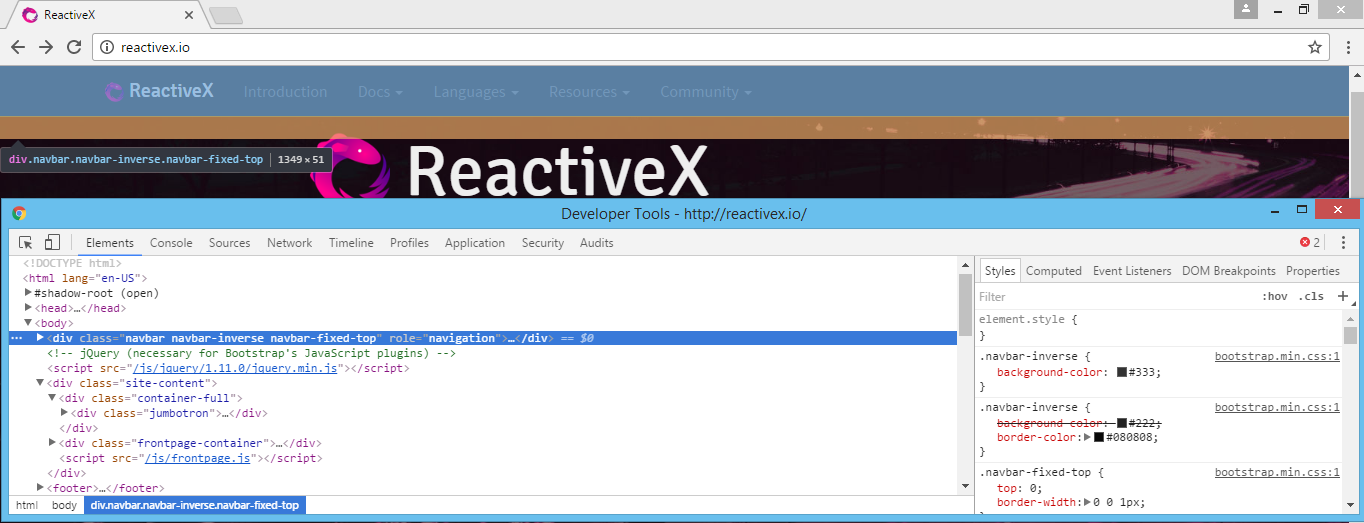
\includegraphics[scale=0.5,trim=0 0 0 0]{gfx/dev_tools.png}
	\caption{Chrome Developer Tools}
	\label{fig:chrome_dev_tools}
	
\end{figure} 

Using the Elements panel, we can see the raw HTML, raw CSS styles, the Document Object Model. One can manipulate HTML or CSS in real time and can see how it is effecting the web page. Web developers use Elements panel quite extensively when they need to inspect HTML and corresponding CSS of part of a web page. This tool also presents minified or ugly HTML in formatted and readable structure. The console panel is used to log and display debugging information along with all errors or warnings generated by the current web page. From the Console panel, we can also enter arbitrary JavaScript and programmatically interact with our page \cite{CCDT}. Web developers especially JavaScript developers use Sources panel to inspect all the JavaScript code that is being used by web page under inspection. One can change running JavaScript code on the fly, one can set breakpoints and can inspect values of variables at runtime \cite{JSDebCDT}. The Network panel can be used for optimization. It provides detailed real-time insights into resources requested and downloaded over the network. More on DevTools can be found from online documentation \cite{CDT}.

\subsection{Extending Chrome DevTools} 	\label{subsec:Extending_Chrome_DevTools}

One does not need to hack Chrome browser code to add functionality to Chrome Devtools. Chrome allows everyone to add functionality to Chrome DevTools by writing extensions to it. To write an extension to DevTools, we need to have knowledge of core web technologies such as HTML, CSS, and JavaScript. We can also distribute our extension by publishing to the Chrome Web Store. By extending DevTools one can add new UI panels and sidebars, interact with the inspected page, get information about network requests, and much more. Dev-Tools extensions have access to a big pool of JavaScript APIs \cite{CDJAPIs} and some DevTools-specific extension APIs. List of sample DevTools extensions can be found here \cite{CDSampExt}.
The manifest file called manifest.json, contains metadata about that particular extension in JSON format. It contains properties like your extension's name, description, version number and so on. At a high level, we will use this file to declare to Chrome what the extension is going to do, and what permissions it requires in order to function properly.
Background page, content script and DevTools page are three main components of DevTools extension as shown in figure~\ref{fig:structure_of_chrome_devtools_extension}. These three components communicate with each other by message passing \cite{CDMesgPassing}.
\begin{figure}[!h]
	\centering
	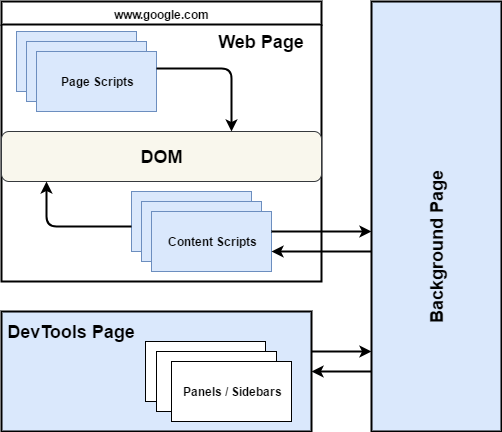
\includegraphics[scale=0.5,trim=0 0 0 0]{gfx/ChromeDevToolsExtension.png}
	\caption{The Structure of Chrome DeveTools Extension}
	\label{fig:structure_of_chrome_devtools_extension}
\end{figure} 
Content Script helps to interact with web pages the browser visits and gives access to shared DOM. The content script is JavaScript code injected by an extension to run in the context of the page that has been loaded into the browser. Content scripts can be injected statically by defining the name of JavaScript file and parameter that tells the extension whether to execute at the start or at the end of the document. The DevTool page can also inject content script dynamically using chrome API. The content script can access and manipulate the DOM of the web page that is currently under inspection. Content script and script belonging to the web page do not conflict with each other because they both execute in an isolated manner.
Background Page is an invisible page that holds the main logic of the extension. Persistent background pages and event pages are two types of background pages to control the behaviour of the extension. Event pages run as needed and persistent background pages run all the time. Besides containing the logic of the extension, background page serve as a communication channel between the inspected page and DevTools page through content scripts.  
The devtools\_page property in the manifest file, must point to an HTML page and that reference to JavaScript file. So DevTools page is not something that you visually need to see, rather it is just something that you need to have in order to run some JavaScript code in DevTools window while it is opened. DevTools page uses devtools APIs, to setup panels/sidebars, to interact with the inspected window and to get information about network requests. DevTools page communicates with the background page using Message Passing.

\section{Related Work}
We split this section into two parts. Firstly, we discuss different perspectives of advancements in debugging techniques, related to our work. In the second part we present some example tools in web domain and aids developers to understand abstraction in the running code.
\subsection{Beyond Traditional Debugging}
%\subsubsection{Omniscient Debuggers}
Log-based debugging and breakpoint-based debugging are two traditional debugging techniques. The first one requires manual modification of source code to trace program execution whereas the second one allows setting breakpoints within the source code to step into code execution. Omniscient debuggers overcome the issues of traditional debuggers and combine the positives of both traditional approaches. During the execution of the program, all events get recorded and presented to the programmer, which can later be used by the developer to see the transformation of states caused by different events \cite{Pothier:2007:SOD:1297105.1297067}. Omniscient debuggers help developers to visualize data and control flow in an application with the ability to navigate forward and backward through the program execution. Besides the powerful advantages of omniscient debuggers, it has some serious concerns regarding performance that is why this technique is not adopted by the software industry as well as in education sector \cite{6983851}. It may require special techniques to process and store events in large, real-world applications. There is a lot of recent research addressing the optimization of omniscient debugging technique  \cite{Pothier:2007:SOD:1297105.1297067,Pothier2011,Lienhard2008}.
Hence, we tried to adopt properties of the omniscient approach in our implementation and thus the pros and cons of this technique also applicable to our work.
%\subsubsection{Object-Centric Debugging}

Traditional debuggers are mostly based on runtime stack information and do not consider any other abstraction within the running code. Object-centric debugging uses objects as abstraction and allow the developer to perform debugging operations based on objects instead of the execution stack \cite{Ressia:2012:OD:2337223.2337280}. Similar to our work, Object-centric debugging is also a representation of the running system. In our case, we focus on declarative abstractions implemented by Reactive Programming paradigm.

\subsection{Related Tools}
%\subsubsection{RxVision}
During this work we have found an application called RxVision \cite{GithubRxvision}, that was made for debugging and visualizing RxJs reactive streams. This tool provides an online web page \cite{PlaygroundRxvision}, where we can write and run RxJS code and can also see a visual representation of that code. This application does not support the latest version of RxJS and was not developed further. The visual representation of RxJs code is very hard to understand and it is very hard to map visual representation to the code because this application does not map event streams to the JavaScript variable. We also looked into the code which is available on GitHub \cite{GithubRxvision}, and we found that they override almost everything of RxJS library to log all internal activities, that is the reason why it does not support the latest version of RxJS.

%\subsubsection{Cycle.js DevTool for Chrome}
Cycle.js DevTool for Chrome is another browser extension which aims to help while debugging and understanding the abstract code \cite{GithubCycleJsDevtool}. This extension is to debug or visualize data flow in Cycle.js \cite{CycleJs} apps. This application has more resemblance to our work because it also displays event stream in the form of dependency graph but this also has the same problem of not getting the reference to the JavaScript variable name. It is not possible to track the history data of streams.

%\subsubsection{React Developer Tools}
React is an open source JavaScript library developed by facebook \cite{ReactFacebook}, for building user interfaces of web applications. Fortunately, this library already has a tool support for debugging, in the form of chrome browser extension \cite{ReactFacebookChrome}. This tool is very helpful for developers to debug the code that is based on React library. Using React dev tool, we can inspect React tree, components and properties passed to each component and the state of each component with some live editing features. This extension is a live and working example that is implemented as a browser extension to explain the abstraction in the code, to the developers.





